\documentclass{standalone}

\usepackage[usenames,dvipsnames]{xcolor}
\usepackage{tikz}
\usepackage{pgfplots}
\usepackage{graphicx}
\usepackage{comment}

\usetikzlibrary{pgfplots.colormaps}

\pgfplotsset{compat=newest}

% Define a custom colormap (continuous gradient)
\pgfplotscreatecolormap{mycolormap}{
	rgb255(0cm)=(0,0,255);      % Blue at start
	rgb255(1cm)=(0,255,0);      % Green in middle
	rgb255(2cm)=(255,0,0)       % Red at end
}

\definecolor{blue1}{RGB}{54,75,154}
\definecolor{blue2}{RGB}{74,123,183}
\definecolor{blue3}{RGB}{110,166,205}
\definecolor{blue4}{RGB}{152,202,225}
\definecolor{blue5}{RGB}{194,228,239}
\definecolor{tan1}{RGB}{234,236,204}
\definecolor{yellow1}{RGB}{254,218,139}
\definecolor{orange1}{RGB}{253,179,102}
\definecolor{orange2}{RGB}{246,126,75}
\definecolor{red1}{RGB}{221,61,45}
\definecolor{red2}{RGB}{165,0,38}

\definecolor{b1}{HTML}{d73027}
\definecolor{b2}{HTML}{fc8d59}
\definecolor{b3}{HTML}{ffffbf}
\definecolor{b4}{HTML}{91bfdb}
\definecolor{b5}{HTML}{4575b4}


\begin{document}
	\vspace{1cm}
		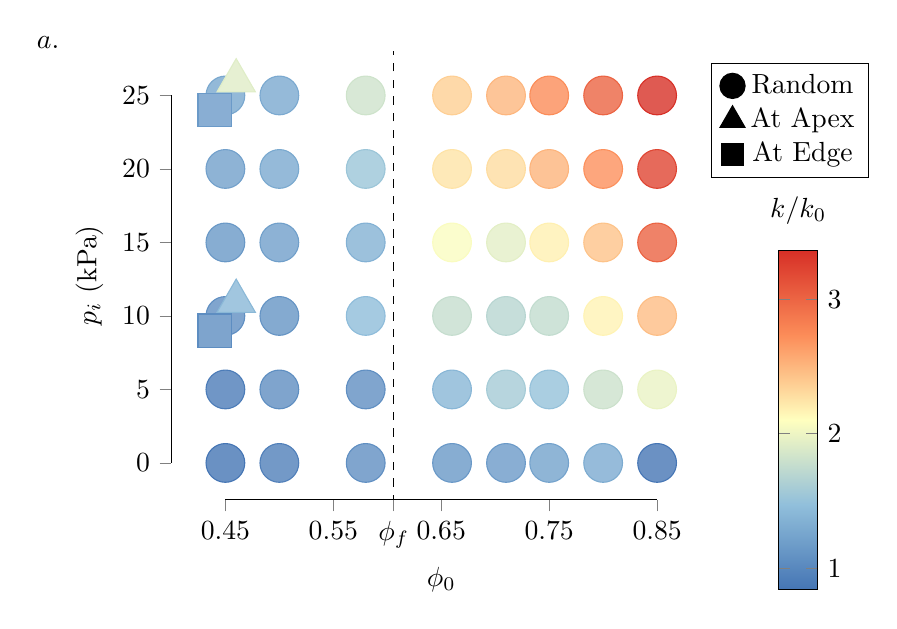
\begin{tikzpicture}
		\begin{axis}[
			%legend style={nodes={scale=0.5, transform shape}},
			%width=8cm,
			title={$a.$},
			title style={yshift=-2ex, xshift=-33ex},
			enlargelimits=false,
			tick pos=left, %
			tick align=outside, %
			axis line style={opacity=0}, %
			after end axis/.code={
				\draw ({rel axis cs:0,0}
				-|{axis cs:0.45,0}) % xmin (line starts here)
				-- ({rel axis cs:0,0}
				-|{axis cs:0.85,0}); % xmax (line stops here)
				\draw ({rel axis cs:0,0}
				|-{axis cs:0,0}) % ymin (line starts here)
				-- ({rel axis cs:0,0}
				|-{axis cs:0,25}); % ymax (line stops here)
			},
			legend image post style={scale=0.65},
			legend style={
				at={(1,0.975)}, % position outside the plot (x=1.05 means 5% to the right)
				anchor=north west,
				/tikz/every even column/.append style={column sep=0.5cm},
			},
			xlabel={$\phi_0$},
			ylabel={$p_i$ (kPa)},
			xmin=0.4,
			xmax=0.9,
			ymin=-2.5,
			ymax=28,
			ytick={0,5,10,15,20,25},
			xtick = {0.45, 0.55, 0.606, 0.65, 0.75, 0.85},
			xticklabels = {0.45, 0.55, \textcolor{black}{$\phi_f$}, 0.65, 0.75, 0.85},
			colorbar, % Show color scale
			colorbar style={
				title={$k/k_0$},
				height = 4.3cm,
				at={(1.125,-0.2)},
				anchor=south west,
			},
			colormap={custom}{
				color(1)=(b5)
				color(2)=(b4)
				color(3)=(b3)
				color(4)=(b2)
				color(5)=(b1)
			},
			%colormap/viridis, % Nice color map
			%point meta min=0.84442789, % Minimum z value
			%point meta max=3.50309299, % Maximum z value
			scatter/use mapped color={draw=mapped color, fill=mapped color!80},
			scatter,
			point meta = explicit,
			mark size=4pt
			]
			%\addlegendimage{empty legend}
			%\addlegendimage{empty legend}
			
			\addplot [scatter, mark = *, mark size = 7 pt, only marks, point meta = explicit]
			table[meta=z] {
				x   y   z
				%0	0	1
				%0	5	1
				%0	10	1
				%0	15	1
				%0	20	1
				%0	25	1
				0.45	0	0.84323997
				0.45	5	0.904955104
				0.45	10	1.065268913
				0.45	15	1.140800423
				0.45	20	1.212309632
				0.45	25	1.270545752
				0.50	0	0.931807817
				0.50	5	1.053849969
				0.50	10	1.109020767
				0.50	15	1.201581008
				0.50	20	1.283995783
				0.50	25	1.288688466
				0.58	0	1.064723137
				0.58	5	1.06399045
				0.58	10	1.45111311
				0.58	15	1.354710003
				0.58	20	1.532471222
				0.58	25	1.825042429
				0.66	0	1.143090691
				0.66	5	1.39798586
				0.66	10	1.772176852
				0.66	15	2.076446121
				0.66	20	2.257848344
				0.66	25	2.36773388
				0.71	0	1.158606699
				0.71	5	1.587639528
				0.71	10	1.691396914
				0.71	15	1.942062936
				0.71	20	2.297129314
				0.71	25	2.50335067
				0.75	0	1.225164045
				0.75	5	1.496457436
				0.75	10	1.753403628
				0.75	15	2.186082445
				0.75	20	2.514208885
				0.75	25	2.74127941
				0.80	0	1.298604656
				0.80	5	1.811118892
				0.80	10	2.169626903
				0.80	15	2.434817065
				0.80	20	2.714436666
				0.80	25	3.011595886
				0.85	0	0.852725021
				0.85	5	1.981368828
				0.85	10	2.466220409
				0.85	15	3.01683933
				0.85	20	3.219648958
				0.85	25	3.360726008
				
			};
			\addplot [scatter, mark = triangle*, mark size = 8pt, only marks, point meta = explicit]
			table[meta=z] {
				x	y	z
				0.46	26	1.920692912
				0.46	11	1.412325582
			};
			\addplot [scatter, mark = square*,mark size = 6 pt, only marks, point meta = explicit]
			table[meta=z] {
				x	y	z
				0.44	24	1.158372439
				0.44	9	1.046171713
			};
			%\addplot [domain=0.3853:0.8377,dashed,,smooth,thick,black,point meta=3,mark=none] {98*x^2 - 177.3*x + 75.5};
			
			\addplot[domain=-5:30, samples=2, dashed, black] ({0.606}, {x});
			
			%\addlegendentry[scale=0.85]{\textbf{Granular}}
			%\addlegendentry[scale=0.85]{\textbf{Arrangement}}
			\addlegendentry[scale=1]{{Random}}
			\addlegendentry[scale=1]{{At Apex}}
			\addlegendentry[scale=1]{{At Edge}}
		\end{axis}
	\end{tikzpicture}

	
\end{document}